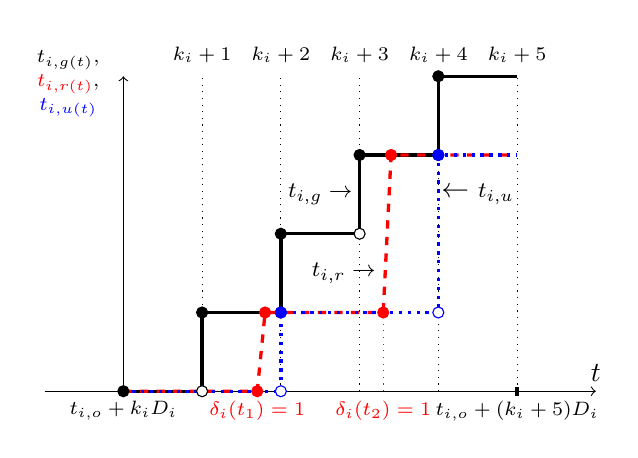
\begin{tikzpicture}

% horizontal axis
\draw[->] (-1,0) -- (6,0) node[anchor=south] {$t$};
% labels
\draw	(0,4.5) node[anchor=east] {}
		(1,4.5) node[anchor=north] {\scriptsize$k_i+1$}
		(2,4.5) node[anchor=north] {\scriptsize$k_i+2$}
		(3,4.5) node[anchor=north] {\scriptsize$k_i+3$}
		(4,4.5) node[anchor=north] {\scriptsize$k_i+4$}
		(5,4.5) node[anchor=north] {\scriptsize$k_i+5$}
		(0,-0.0) node[anchor=north]
		{\scriptsize$t_{i,o} + k_i D_i$}
		(5,-0.0) node[anchor=north]
		{\scriptsize$t_{i,o}+(k_i+5)D_i$}
		(1.7,-0.0) node[anchor=north] {\color{red}\scriptsize$\delta_i(t_1)=1$}
		(3.3,-0.0) node[anchor=north] {\color{red}\scriptsize$\delta_i(t_2)=1$};

\node[] at (-0.7, 4.2) {\scriptsize$t_{i,g(t)}$,};
\node[] at (-0.7, 3.9) {\color{red}{\scriptsize$t_{i,r(t)}$}\color{black}{\scriptsize,}};
\node[] at (-0.7, 3.6) {\color{blue}{\scriptsize$t_{i,u(t)}$}};

\draw[very thick, black] (5,-0.06) --  (5,+0.06);
	
% vertical axis
\draw[->] (0,0) -- (0,4) node[anchor=east] {};
% vertical ticks
\draw[dotted] (1,0) -- (1,4);
\draw[dotted] (2,0) -- (2,4);
\draw[dotted] (3,0) -- (3,4);
\draw[dotted] (4,0) -- (4,4);
\draw[dotted] (5,0) -- (5,4);
\draw[dotted,red] (3.3,0) -- (3.3,1);

% Delta 1
%\draw[very thick, black, solid] (0,1) -- (1,1);
%\draw[very thick, black, solid] (1,0) -- (2,0);
%\draw[very thick, black, solid] (2,1) -- (3,1);
%\draw[very thick, black, solid] (3,2) -- (4,2);
%\draw[very thick, black, solid] (0,1) -- (1,1);
%\draw[very thick, black, solid] (0,1) -- (1,1);
\draw[very thick, black, solid] (0,0) --  (1,0) -- (1,1) -- (2,1) -- (2,2) -- (3,2) --  (3,3) -- (4,3) -- (4,4)-- (5,4);

\draw[very thick, red, dashed] (0,0) --  (1.7,0) -- (1.8,1) -- (3.3,1) -- (3.4,3) -- (5,3);

\draw[very thick, blue, dotted] (0,0) --  (2,0) -- (2,1) -- (4,1) -- (4,3) -- (5,3);

%\draw (-.7, 1) node {\scriptsize$\Delta[k-1]$}; %label
\draw (2.5, 2.5) node { \footnotesize$t_{i,g}\rightarrow$};

\draw (2.8, 1.5) node { \footnotesize$t_{i,r}\rightarrow$};

\draw (4.5, 2.5) node { $\leftarrow\,\,$\footnotesize$t_{i,u}$};



\node[circle,draw=black, fill=white, inner sep=0pt,minimum size=4pt] (b) at (1,0) {};
\node[circle,draw=black, fill=white, inner sep=0pt,minimum size=4pt] (b) at (2,1) {};
\node[circle,draw=black, fill=white, inner sep=0pt,minimum size=4pt] (b) at (3,2) {};
\node[circle,draw=black, fill=white, inner sep=0pt,minimum size=4pt] (b) at (4,3) {};


\node[circle,draw=black, fill=black, inner sep=0pt,minimum size=4pt] (b) at (0,0) {};
\node[circle,draw=black, fill=black, inner sep=0pt,minimum size=4pt] (b) at (1,1) {};
\node[circle,draw=black, fill=black, inner sep=0pt,minimum size=4pt] (b) at (2,2) {};
\node[circle,draw=black, fill=black, inner sep=0pt,minimum size=4pt] (b) at (3,3) {};
\node[circle,draw=black, fill=black, inner sep=0pt,minimum size=4pt] (b) at (4,4) {};
%\node[circle,draw=black, fill=black, inner sep=0pt,minimum size=4pt] (b) at (5,4) {};

\node[circle,draw=blue, fill=white, inner sep=0pt,minimum size=4pt] (b) at (2,0) {};
\node[circle,draw=blue, fill=white, inner sep=0pt,minimum size=4pt] (b) at (4,1) {};



\node[circle,draw=blue, fill=blue, inner sep=0pt,minimum size=4pt] (b) at (2,1) {};
\node[circle,draw=blue, fill=blue, inner sep=0pt,minimum size=4pt] (b) at (4,3) {};


\node[circle,draw=red, fill=red, inner sep=0pt,minimum size=4pt] (b) at (1.7,0) {};
\node[circle,draw=red, fill=red, inner sep=0pt,minimum size=4pt] (b) at (3.3,1) {};



\node[circle,draw=red, fill=red, inner sep=0pt,minimum size=4pt] (b) at (1.8,1) {};
\node[circle,draw=red, fill=red, inner sep=0pt,minimum size=4pt] (b) at (3.4,3) {};


\end{tikzpicture}
